% Figure 1: Keel's pipeline (top) beside LLM-extraction memories (bottom).
% Build: tectonic fig1-architecture.tex
\documentclass[tikz,border=1pt]{standalone}
\usepackage[T1]{fontenc}
\usepackage{DejaVuSans}
\renewcommand{\familydefault}{\sfdefault}
\usetikzlibrary{arrows.meta,positioning,calc,fit,backgrounds}
\hyphenpenalty=10000 \exhyphenpenalty=10000

\definecolor{keel}{HTML}{2a78d6}
\definecolor{keelwash}{HTML}{e3eefb}
\definecolor{ink}{HTML}{0b0b0b}
\definecolor{inktwo}{HTML}{52514e}
\definecolor{muted}{HTML}{898781}
\definecolor{rule}{HTML}{c3c2b7}
\definecolor{lanerule}{HTML}{dcdad2}

\newcommand{\h}[1]{{\fontsize{7.2}{8.5}\selectfont\bfseries\color{ink}#1}}

\begin{document}
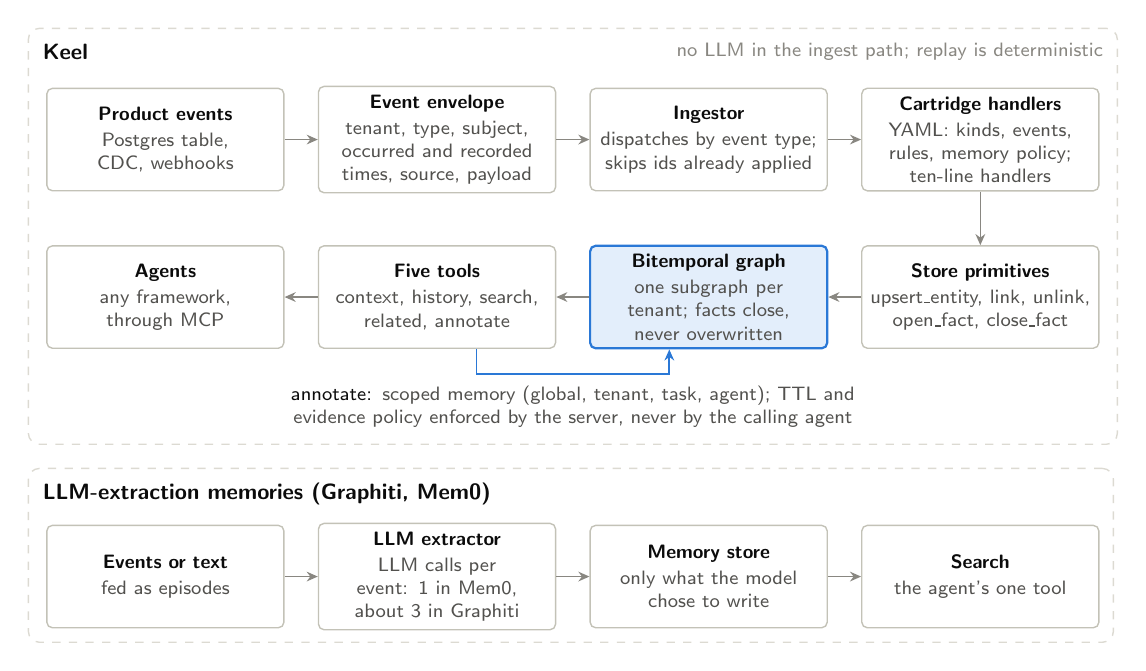
\begin{tikzpicture}[
  font=\fontsize{7}{8.4}\selectfont, text=inktwo,
  box/.style={draw=rule, line width=0.5pt, rounded corners=2pt, fill=white,
              text width=2.8cm, align=center, inner sep=3pt, minimum height=1.3cm},
  hl/.style={box, draw=keel, line width=0.8pt, fill=keelwash},
  flow/.style={-{Stealth[length=4pt,width=3.5pt]}, draw=muted, line width=0.6pt},
  back/.style={-{Stealth[length=4pt,width=3.5pt]}, draw=keel, line width=0.6pt},
  lane/.style={draw=lanerule, dashed, rounded corners=4pt, line width=0.5pt, inner sep=5pt},
  lanetitle/.style={font=\fontsize{8}{9.5}\selectfont\bfseries, text=ink, anchor=west, inner sep=0pt},
]
\def\dx{3.45}

% ---- Keel lane, row 1 (ingest)
\node[box] (ev)   at (0,0)      {\h{Product events}\\[1pt] Postgres table, CDC, webhooks};
\node[box] (env)  at (\dx,0)    {\h{Event envelope}\\[1pt] tenant, type, subject, occurred and recorded times, source, payload};
\node[box] (ing)  at (2*\dx,0)  {\h{Ingestor}\\[1pt] dispatches by event type; skips ids already applied};
\node[box] (hand) at (3*\dx,0)  {\h{Cartridge handlers}\\[1pt] YAML: kinds, events, rules, memory policy; ten-line handlers};

% ---- Keel lane, row 2 (read and write back), right to left
\node[box] (prim)  at (3*\dx,-2.0) {\h{Store primitives}\\[1pt] upsert\_entity, link, unlink, open\_fact, close\_fact};
\node[hl]  (graph) at (2*\dx,-2.0) {\h{Bitemporal graph}\\[1pt] one subgraph per tenant; facts close, never overwritten};
\node[box] (tools) at (\dx,-2.0)   {\h{Five tools}\\[1pt] context, history, search, related, annotate};
\node[box] (agents) at (0,-2.0)    {\h{Agents}\\[1pt] any framework, through MCP};

\draw[flow] (ev) -- (env);
\draw[flow] (env) -- (ing);
\draw[flow] (ing) -- (hand);
\draw[flow] (hand) -- (prim);
\draw[flow] (prim) -- (graph);
\draw[flow] (graph) -- (tools);
\draw[flow] (tools) -- (agents);

% annotate: the only write path from the tools back into the graph
\draw[back] ([xshift=0.5cm]tools.south) -- ++(0,-0.32) -| ([xshift=-0.5cm]graph.south);
\node[text width=7.2cm, align=center, anchor=north, inner sep=1pt]
  (annot) at ($(tools.south)!0.5!(graph.south) + (0,-0.42)$)
  {{\color{ink}annotate:} scoped memory (global, tenant, task, agent); TTL and evidence policy enforced by the server, never by the calling agent};

\node[lanetitle] (ktitle) at ([xshift=-0.05cm, yshift=1.12cm]ev.west) {Keel};
\node[anchor=east, inner sep=0pt, text=muted] (knote) at ([xshift=0.05cm, yshift=1.12cm]hand.east)
  {no LLM in the ingest path; replay is deterministic};

\begin{scope}[on background layer]
  \node[lane, fit=(ev)(hand)(agents)(prim)(annot)(ktitle)(knote)] (keellane) {};
\end{scope}

% ---- LLM-extraction lane
\def\ly{-5.55}
\node[box] (x1) at (0,\ly)      {\h{Events or text}\\[1pt] fed as episodes};
\node[box] (x2) at (\dx,\ly)    {\h{LLM extractor}\\[1pt] LLM calls per event: 1 in Mem0, about 3 in Graphiti};
\node[box] (x3) at (2*\dx,\ly)  {\h{Memory store}\\[1pt] only what the model chose to write};
\node[box] (x4) at (3*\dx,\ly)  {\h{Search}\\[1pt] the agent's one tool};
\draw[flow] (x1) -- (x2);
\draw[flow] (x2) -- (x3);
\draw[flow] (x3) -- (x4);

\node[lanetitle] (ltitle) at ([xshift=-0.05cm, yshift=1.05cm]x1.west) {LLM-extraction memories (Graphiti, Mem0)};
\begin{scope}[on background layer]
  \node[lane, fit=(x1)(x4)(ltitle)] (llmlane) {};
\end{scope}

\end{tikzpicture}
\end{document}
